\documentclass[twoside]{book}

% Packages required by doxygen
\usepackage{fixltx2e}
\usepackage{calc}
\usepackage{doxygen}
\usepackage[export]{adjustbox} % also loads graphicx
\usepackage{graphicx}
\usepackage[utf8]{inputenc}
\usepackage{makeidx}
\usepackage{multicol}
\usepackage{multirow}
\PassOptionsToPackage{warn}{textcomp}
\usepackage{textcomp}
\usepackage[nointegrals]{wasysym}
\usepackage[table]{xcolor}

% Font selection
\usepackage[T1]{fontenc}
\usepackage[scaled=.90]{helvet}
\usepackage{courier}
\usepackage{amssymb}
\usepackage{sectsty}
\renewcommand{\familydefault}{\sfdefault}
\allsectionsfont{%
  \fontseries{bc}\selectfont%
  \color{darkgray}%
}
\renewcommand{\DoxyLabelFont}{%
  \fontseries{bc}\selectfont%
  \color{darkgray}%
}
\newcommand{\+}{\discretionary{\mbox{\scriptsize$\hookleftarrow$}}{}{}}

% Page & text layout
\usepackage{geometry}
\geometry{%
  a4paper,%
  top=2.5cm,%
  bottom=2.5cm,%
  left=2.5cm,%
  right=2.5cm%
}
\tolerance=750
\hfuzz=15pt
\hbadness=750
\setlength{\emergencystretch}{15pt}
\setlength{\parindent}{0cm}
\setlength{\parskip}{3ex plus 2ex minus 2ex}
\makeatletter
\renewcommand{\paragraph}{%
  \@startsection{paragraph}{4}{0ex}{-1.0ex}{1.0ex}{%
    \normalfont\normalsize\bfseries\SS@parafont%
  }%
}
\renewcommand{\subparagraph}{%
  \@startsection{subparagraph}{5}{0ex}{-1.0ex}{1.0ex}{%
    \normalfont\normalsize\bfseries\SS@subparafont%
  }%
}
\makeatother

% Headers & footers
\usepackage{fancyhdr}
\pagestyle{fancyplain}
\fancyhead[LE]{\fancyplain{}{\bfseries\thepage}}
\fancyhead[CE]{\fancyplain{}{}}
\fancyhead[RE]{\fancyplain{}{\bfseries\leftmark}}
\fancyhead[LO]{\fancyplain{}{\bfseries\rightmark}}
\fancyhead[CO]{\fancyplain{}{}}
\fancyhead[RO]{\fancyplain{}{\bfseries\thepage}}
\fancyfoot[LE]{\fancyplain{}{}}
\fancyfoot[CE]{\fancyplain{}{}}
\fancyfoot[RE]{\fancyplain{}{\bfseries\scriptsize Generated by Doxygen }}
\fancyfoot[LO]{\fancyplain{}{\bfseries\scriptsize Generated by Doxygen }}
\fancyfoot[CO]{\fancyplain{}{}}
\fancyfoot[RO]{\fancyplain{}{}}
\renewcommand{\footrulewidth}{0.4pt}
\renewcommand{\chaptermark}[1]{%
  \markboth{#1}{}%
}
\renewcommand{\sectionmark}[1]{%
  \markright{\thesection\ #1}%
}

% Indices & bibliography
\usepackage{natbib}
\usepackage[titles]{tocloft}
\setcounter{tocdepth}{3}
\setcounter{secnumdepth}{5}
\makeindex

% Hyperlinks (required, but should be loaded last)
\usepackage{ifpdf}
\ifpdf
  \usepackage[pdftex,pagebackref=true]{hyperref}
\else
  \usepackage[ps2pdf,pagebackref=true]{hyperref}
\fi
\hypersetup{%
  colorlinks=true,%
  linkcolor=blue,%
  citecolor=blue,%
  unicode%
}

% Custom commands
\newcommand{\clearemptydoublepage}{%
  \newpage{\pagestyle{empty}\cleardoublepage}%
}

\usepackage{caption}
\captionsetup{labelsep=space,justification=centering,font={bf},singlelinecheck=off,skip=4pt,position=top}

%===== C O N T E N T S =====

\begin{document}

% Titlepage & ToC
\hypersetup{pageanchor=false,
             bookmarksnumbered=true,
             pdfencoding=unicode
            }
\pagenumbering{alph}
\begin{titlepage}
\vspace*{7cm}
\begin{center}%
{\Large My Project }\\
\vspace*{1cm}
{\large Generated by Doxygen 1.8.14}\\
\end{center}
\end{titlepage}
\clearemptydoublepage
\pagenumbering{roman}
\tableofcontents
\clearemptydoublepage
\pagenumbering{arabic}
\hypersetup{pageanchor=true}

%--- Begin generated contents ---
\chapter{Hierarchical Index}
\section{Class Hierarchy}
This inheritance list is sorted roughly, but not completely, alphabetically\+:\begin{DoxyCompactList}
\item A\+Actor\begin{DoxyCompactList}
\item \contentsline{section}{A\+My\+Weapon\+\_\+\+Gun}{\pageref{class_a_my_weapon___gun}}{}
\begin{DoxyCompactList}
\item \contentsline{section}{A\+Rocket\+Launcher}{\pageref{class_a_rocket_launcher}}{}
\item \contentsline{section}{A\+S\+Projectile\+Weapon}{\pageref{class_a_s_projectile_weapon}}{}
\end{DoxyCompactList}
\end{DoxyCompactList}
\item A\+Character\begin{DoxyCompactList}
\item \contentsline{section}{A\+Instructor\+Of\+The\+Dead2\+Character}{\pageref{class_a_instructor_of_the_dead2_character}}{}
\item \contentsline{section}{A\+Main\+Character}{\pageref{class_a_main_character}}{}
\end{DoxyCompactList}
\item A\+Game\+Mode\+Base\begin{DoxyCompactList}
\item \contentsline{section}{A\+Instructor\+Of\+The\+Dead2\+Game\+Mode}{\pageref{class_a_instructor_of_the_dead2_game_mode}}{}
\end{DoxyCompactList}
\item A\+Trigger\+Volume\begin{DoxyCompactList}
\item \contentsline{section}{A\+Level\+Boundary}{\pageref{class_a_level_boundary}}{}
\end{DoxyCompactList}
\item \contentsline{section}{F\+Hit\+Scan\+Trace}{\pageref{struct_f_hit_scan_trace}}{}
\item I\+Module\+Interface\begin{DoxyCompactList}
\item \contentsline{section}{F\+Testing\+Module}{\pageref{class_f_testing_module}}{}
\end{DoxyCompactList}
\item \contentsline{section}{Level\+Boundary\+Test}{\pageref{class_level_boundary_test}}{}
\item \contentsline{section}{Level\+Boundary\+Test2}{\pageref{class_level_boundary_test2}}{}
\item Module\+Rules\begin{DoxyCompactList}
\item \contentsline{section}{Instructor\+Of\+The\+Dead2}{\pageref{class_instructor_of_the_dead2}}{}
\item \contentsline{section}{Testing\+Module}{\pageref{class_testing_module}}{}
\end{DoxyCompactList}
\item \contentsline{section}{My\+Health\+Component\+Testing}{\pageref{class_my_health_component_testing}}{}
\item \contentsline{section}{My\+Weapon\+\_\+\+Gun\+Test1}{\pageref{class_my_weapon___gun_test1}}{}
\item \contentsline{section}{My\+Weapon\+\_\+\+Gun\+Test2}{\pageref{class_my_weapon___gun_test2}}{}
\item \contentsline{section}{My\+Weapon\+\_\+\+Gun\+Test3}{\pageref{class_my_weapon___gun_test3}}{}
\item \contentsline{section}{My\+Weapon\+\_\+\+Gun\+Test4}{\pageref{class_my_weapon___gun_test4}}{}
\item \contentsline{section}{My\+Weapon\+\_\+\+Gun\+Test5}{\pageref{class_my_weapon___gun_test5}}{}
\item \contentsline{section}{Rocket\+Launcher\+Test}{\pageref{class_rocket_launcher_test}}{}
\item \contentsline{section}{Rocket\+Launcher\+Test2}{\pageref{class_rocket_launcher_test2}}{}
\item \contentsline{section}{Rocket\+Launcher\+Test3}{\pageref{class_rocket_launcher_test3}}{}
\item \contentsline{section}{Rocket\+Launcher\+Test4}{\pageref{class_rocket_launcher_test4}}{}
\item \contentsline{section}{Steam\+Test}{\pageref{class_steam_test}}{}
\item Target\+Rules\begin{DoxyCompactList}
\item \contentsline{section}{Instructor\+Of\+The\+Dead2\+Editor\+Target}{\pageref{class_instructor_of_the_dead2_editor_target}}{}
\item \contentsline{section}{Instructor\+Of\+The\+Dead2\+Target}{\pageref{class_instructor_of_the_dead2_target}}{}
\end{DoxyCompactList}
\end{DoxyCompactList}

\chapter{Class Index}
\section{Class List}
Here are the classes, structs, unions and interfaces with brief descriptions\+:\begin{DoxyCompactList}
\item\contentsline{section}{\mbox{\hyperlink{class_a_instructor_of_the_dead2_character}{A\+Instructor\+Of\+The\+Dead2\+Character}} }{\pageref{class_a_instructor_of_the_dead2_character}}{}
\item\contentsline{section}{\mbox{\hyperlink{class_a_instructor_of_the_dead2_game_mode}{A\+Instructor\+Of\+The\+Dead2\+Game\+Mode}} }{\pageref{class_a_instructor_of_the_dead2_game_mode}}{}
\item\contentsline{section}{\mbox{\hyperlink{class_a_level_boundary}{A\+Level\+Boundary}} }{\pageref{class_a_level_boundary}}{}
\item\contentsline{section}{\mbox{\hyperlink{class_a_main_character}{A\+Main\+Character}} }{\pageref{class_a_main_character}}{}
\item\contentsline{section}{\mbox{\hyperlink{class_a_my_weapon___gun}{A\+My\+Weapon\+\_\+\+Gun}} }{\pageref{class_a_my_weapon___gun}}{}
\item\contentsline{section}{\mbox{\hyperlink{class_a_rocket_launcher}{A\+Rocket\+Launcher}} }{\pageref{class_a_rocket_launcher}}{}
\item\contentsline{section}{\mbox{\hyperlink{class_a_s_projectile_weapon}{A\+S\+Projectile\+Weapon}} }{\pageref{class_a_s_projectile_weapon}}{}
\item\contentsline{section}{\mbox{\hyperlink{struct_f_hit_scan_trace}{F\+Hit\+Scan\+Trace}} }{\pageref{struct_f_hit_scan_trace}}{}
\item\contentsline{section}{\mbox{\hyperlink{class_f_testing_module}{F\+Testing\+Module}} }{\pageref{class_f_testing_module}}{}
\item\contentsline{section}{\mbox{\hyperlink{class_instructor_of_the_dead2}{Instructor\+Of\+The\+Dead2}} }{\pageref{class_instructor_of_the_dead2}}{}
\item\contentsline{section}{\mbox{\hyperlink{class_instructor_of_the_dead2_editor_target}{Instructor\+Of\+The\+Dead2\+Editor\+Target}} }{\pageref{class_instructor_of_the_dead2_editor_target}}{}
\item\contentsline{section}{\mbox{\hyperlink{class_instructor_of_the_dead2_target}{Instructor\+Of\+The\+Dead2\+Target}} }{\pageref{class_instructor_of_the_dead2_target}}{}
\item\contentsline{section}{\mbox{\hyperlink{class_level_boundary_test}{Level\+Boundary\+Test}} }{\pageref{class_level_boundary_test}}{}
\item\contentsline{section}{\mbox{\hyperlink{class_level_boundary_test2}{Level\+Boundary\+Test2}} }{\pageref{class_level_boundary_test2}}{}
\item\contentsline{section}{\mbox{\hyperlink{class_my_health_component_testing}{My\+Health\+Component\+Testing}} }{\pageref{class_my_health_component_testing}}{}
\item\contentsline{section}{\mbox{\hyperlink{class_my_weapon___gun_test1}{My\+Weapon\+\_\+\+Gun\+Test1}} }{\pageref{class_my_weapon___gun_test1}}{}
\item\contentsline{section}{\mbox{\hyperlink{class_my_weapon___gun_test2}{My\+Weapon\+\_\+\+Gun\+Test2}} }{\pageref{class_my_weapon___gun_test2}}{}
\item\contentsline{section}{\mbox{\hyperlink{class_my_weapon___gun_test3}{My\+Weapon\+\_\+\+Gun\+Test3}} }{\pageref{class_my_weapon___gun_test3}}{}
\item\contentsline{section}{\mbox{\hyperlink{class_my_weapon___gun_test4}{My\+Weapon\+\_\+\+Gun\+Test4}} }{\pageref{class_my_weapon___gun_test4}}{}
\item\contentsline{section}{\mbox{\hyperlink{class_my_weapon___gun_test5}{My\+Weapon\+\_\+\+Gun\+Test5}} }{\pageref{class_my_weapon___gun_test5}}{}
\item\contentsline{section}{\mbox{\hyperlink{class_rocket_launcher_test}{Rocket\+Launcher\+Test}} }{\pageref{class_rocket_launcher_test}}{}
\item\contentsline{section}{\mbox{\hyperlink{class_rocket_launcher_test2}{Rocket\+Launcher\+Test2}} }{\pageref{class_rocket_launcher_test2}}{}
\item\contentsline{section}{\mbox{\hyperlink{class_rocket_launcher_test3}{Rocket\+Launcher\+Test3}} }{\pageref{class_rocket_launcher_test3}}{}
\item\contentsline{section}{\mbox{\hyperlink{class_rocket_launcher_test4}{Rocket\+Launcher\+Test4}} }{\pageref{class_rocket_launcher_test4}}{}
\item\contentsline{section}{\mbox{\hyperlink{class_steam_test}{Steam\+Test}} }{\pageref{class_steam_test}}{}
\item\contentsline{section}{\mbox{\hyperlink{class_testing_module}{Testing\+Module}} }{\pageref{class_testing_module}}{}
\end{DoxyCompactList}

\chapter{Class Documentation}
\hypertarget{class_a_instructor_of_the_dead2_character}{}\section{A\+Instructor\+Of\+The\+Dead2\+Character Class Reference}
\label{class_a_instructor_of_the_dead2_character}\index{A\+Instructor\+Of\+The\+Dead2\+Character@{A\+Instructor\+Of\+The\+Dead2\+Character}}
Inheritance diagram for A\+Instructor\+Of\+The\+Dead2\+Character\+:\begin{figure}[H]
\begin{center}
\leavevmode
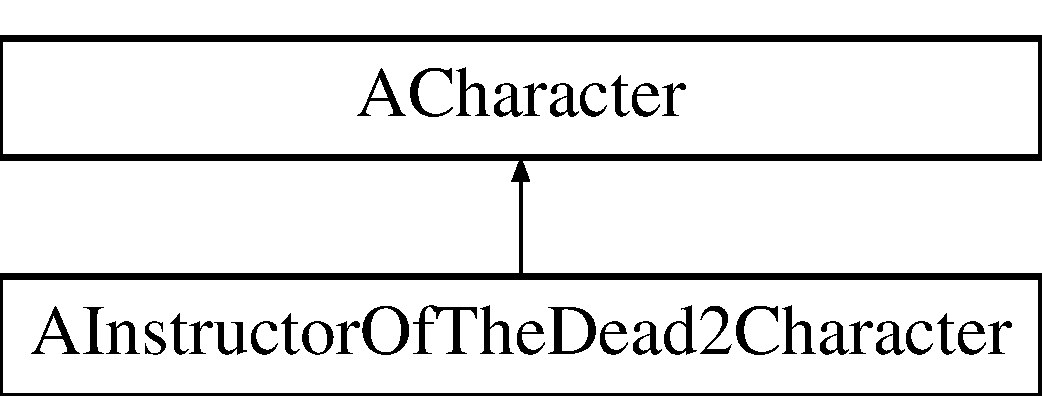
\includegraphics[height=2.000000cm]{class_a_instructor_of_the_dead2_character}
\end{center}
\end{figure}
\subsection*{Public Member Functions}
\begin{DoxyCompactItemize}
\item 
\mbox{\Hypertarget{class_a_instructor_of_the_dead2_character_a4b8d6b1af2b365ed2a3cf737d22ba55b}\label{class_a_instructor_of_the_dead2_character_a4b8d6b1af2b365ed2a3cf737d22ba55b}} 
virtual F\+Vector {\bfseries Get\+Pawn\+View\+Location} () const override
\item 
F\+O\+R\+C\+E\+I\+N\+L\+I\+NE class U\+Spring\+Arm\+Component $\ast$ \mbox{\hyperlink{class_a_instructor_of_the_dead2_character_ad5bcd22697b38d057ef996ccb70dc764}{Get\+Camera\+Boom}} () const
\item 
F\+O\+R\+C\+E\+I\+N\+L\+I\+NE class U\+Camera\+Component $\ast$ \mbox{\hyperlink{class_a_instructor_of_the_dead2_character_a8f18771c845fc64a4446f294e7e6900a}{Get\+Follow\+Camera}} () const
\end{DoxyCompactItemize}
\subsection*{Public Attributes}
\begin{DoxyCompactItemize}
\item 
float \mbox{\hyperlink{class_a_instructor_of_the_dead2_character_a145d6b8d0339f10ea25c4fc746b190c2}{Base\+Turn\+Rate}}
\item 
float \mbox{\hyperlink{class_a_instructor_of_the_dead2_character_ab286e704f971b49ef302350c50491b19}{Base\+Look\+Up\+Rate}}
\end{DoxyCompactItemize}
\subsection*{Protected Member Functions}
\begin{DoxyCompactItemize}
\item 
void \mbox{\hyperlink{class_a_instructor_of_the_dead2_character_a0184954967f084a32645f6a922b9abf6}{On\+Reset\+VR}} ()
\item 
void \mbox{\hyperlink{class_a_instructor_of_the_dead2_character_abcb6cf374cdbe25d392fcc8f200aabc4}{Move\+Forward}} (float Value)
\item 
void \mbox{\hyperlink{class_a_instructor_of_the_dead2_character_aef03c889b18601bafcbae9ae599fafaa}{Move\+Right}} (float Value)
\item 
void \mbox{\hyperlink{class_a_instructor_of_the_dead2_character_a1aa71be0ce8a17e242cbe1f6d41bf905}{Turn\+At\+Rate}} (float Rate)
\item 
void \mbox{\hyperlink{class_a_instructor_of_the_dead2_character_a85db2f08175143a34e1d72304348a840}{Look\+Up\+At\+Rate}} (float Rate)
\item 
void \mbox{\hyperlink{class_a_instructor_of_the_dead2_character_aaf275b2c17de5ce577aa5a0e4202b222}{Touch\+Started}} (E\+Touch\+Index\+::\+Type Finger\+Index, F\+Vector Location)
\item 
void \mbox{\hyperlink{class_a_instructor_of_the_dead2_character_af518d02c1c15d184cd2e75a7aad9b6a5}{Touch\+Stopped}} (E\+Touch\+Index\+::\+Type Finger\+Index, F\+Vector Location)
\item 
\mbox{\Hypertarget{class_a_instructor_of_the_dead2_character_adc1403fc3d4bc95aa169cf73bacf2d04}\label{class_a_instructor_of_the_dead2_character_adc1403fc3d4bc95aa169cf73bacf2d04}} 
virtual void {\bfseries Setup\+Player\+Input\+Component} (class U\+Input\+Component $\ast$Player\+Input\+Component) override
\end{DoxyCompactItemize}


\subsection{Member Function Documentation}
\mbox{\Hypertarget{class_a_instructor_of_the_dead2_character_ad5bcd22697b38d057ef996ccb70dc764}\label{class_a_instructor_of_the_dead2_character_ad5bcd22697b38d057ef996ccb70dc764}} 
\index{A\+Instructor\+Of\+The\+Dead2\+Character@{A\+Instructor\+Of\+The\+Dead2\+Character}!Get\+Camera\+Boom@{Get\+Camera\+Boom}}
\index{Get\+Camera\+Boom@{Get\+Camera\+Boom}!A\+Instructor\+Of\+The\+Dead2\+Character@{A\+Instructor\+Of\+The\+Dead2\+Character}}
\subsubsection{\texorpdfstring{Get\+Camera\+Boom()}{GetCameraBoom()}}
{\footnotesize\ttfamily F\+O\+R\+C\+E\+I\+N\+L\+I\+NE class U\+Spring\+Arm\+Component$\ast$ A\+Instructor\+Of\+The\+Dead2\+Character\+::\+Get\+Camera\+Boom (\begin{DoxyParamCaption}{ }\end{DoxyParamCaption}) const\hspace{0.3cm}{\ttfamily [inline]}}

Returns Camera\+Boom subobject \mbox{\Hypertarget{class_a_instructor_of_the_dead2_character_a8f18771c845fc64a4446f294e7e6900a}\label{class_a_instructor_of_the_dead2_character_a8f18771c845fc64a4446f294e7e6900a}} 
\index{A\+Instructor\+Of\+The\+Dead2\+Character@{A\+Instructor\+Of\+The\+Dead2\+Character}!Get\+Follow\+Camera@{Get\+Follow\+Camera}}
\index{Get\+Follow\+Camera@{Get\+Follow\+Camera}!A\+Instructor\+Of\+The\+Dead2\+Character@{A\+Instructor\+Of\+The\+Dead2\+Character}}
\subsubsection{\texorpdfstring{Get\+Follow\+Camera()}{GetFollowCamera()}}
{\footnotesize\ttfamily F\+O\+R\+C\+E\+I\+N\+L\+I\+NE class U\+Camera\+Component$\ast$ A\+Instructor\+Of\+The\+Dead2\+Character\+::\+Get\+Follow\+Camera (\begin{DoxyParamCaption}{ }\end{DoxyParamCaption}) const\hspace{0.3cm}{\ttfamily [inline]}}

Returns Follow\+Camera subobject \mbox{\Hypertarget{class_a_instructor_of_the_dead2_character_a85db2f08175143a34e1d72304348a840}\label{class_a_instructor_of_the_dead2_character_a85db2f08175143a34e1d72304348a840}} 
\index{A\+Instructor\+Of\+The\+Dead2\+Character@{A\+Instructor\+Of\+The\+Dead2\+Character}!Look\+Up\+At\+Rate@{Look\+Up\+At\+Rate}}
\index{Look\+Up\+At\+Rate@{Look\+Up\+At\+Rate}!A\+Instructor\+Of\+The\+Dead2\+Character@{A\+Instructor\+Of\+The\+Dead2\+Character}}
\subsubsection{\texorpdfstring{Look\+Up\+At\+Rate()}{LookUpAtRate()}}
{\footnotesize\ttfamily void A\+Instructor\+Of\+The\+Dead2\+Character\+::\+Look\+Up\+At\+Rate (\begin{DoxyParamCaption}\item[{float}]{Rate }\end{DoxyParamCaption})\hspace{0.3cm}{\ttfamily [protected]}}

Called via input to turn look up/down at a given rate. 
\begin{DoxyParams}{Parameters}
{\em Rate} & This is a normalized rate, i.\+e. 1.\+0 means 100\% of desired turn rate \\
\hline
\end{DoxyParams}
\mbox{\Hypertarget{class_a_instructor_of_the_dead2_character_abcb6cf374cdbe25d392fcc8f200aabc4}\label{class_a_instructor_of_the_dead2_character_abcb6cf374cdbe25d392fcc8f200aabc4}} 
\index{A\+Instructor\+Of\+The\+Dead2\+Character@{A\+Instructor\+Of\+The\+Dead2\+Character}!Move\+Forward@{Move\+Forward}}
\index{Move\+Forward@{Move\+Forward}!A\+Instructor\+Of\+The\+Dead2\+Character@{A\+Instructor\+Of\+The\+Dead2\+Character}}
\subsubsection{\texorpdfstring{Move\+Forward()}{MoveForward()}}
{\footnotesize\ttfamily void A\+Instructor\+Of\+The\+Dead2\+Character\+::\+Move\+Forward (\begin{DoxyParamCaption}\item[{float}]{Value }\end{DoxyParamCaption})\hspace{0.3cm}{\ttfamily [protected]}}

Called for forwards/backward input \mbox{\Hypertarget{class_a_instructor_of_the_dead2_character_aef03c889b18601bafcbae9ae599fafaa}\label{class_a_instructor_of_the_dead2_character_aef03c889b18601bafcbae9ae599fafaa}} 
\index{A\+Instructor\+Of\+The\+Dead2\+Character@{A\+Instructor\+Of\+The\+Dead2\+Character}!Move\+Right@{Move\+Right}}
\index{Move\+Right@{Move\+Right}!A\+Instructor\+Of\+The\+Dead2\+Character@{A\+Instructor\+Of\+The\+Dead2\+Character}}
\subsubsection{\texorpdfstring{Move\+Right()}{MoveRight()}}
{\footnotesize\ttfamily void A\+Instructor\+Of\+The\+Dead2\+Character\+::\+Move\+Right (\begin{DoxyParamCaption}\item[{float}]{Value }\end{DoxyParamCaption})\hspace{0.3cm}{\ttfamily [protected]}}

Called for side to side input \mbox{\Hypertarget{class_a_instructor_of_the_dead2_character_a0184954967f084a32645f6a922b9abf6}\label{class_a_instructor_of_the_dead2_character_a0184954967f084a32645f6a922b9abf6}} 
\index{A\+Instructor\+Of\+The\+Dead2\+Character@{A\+Instructor\+Of\+The\+Dead2\+Character}!On\+Reset\+VR@{On\+Reset\+VR}}
\index{On\+Reset\+VR@{On\+Reset\+VR}!A\+Instructor\+Of\+The\+Dead2\+Character@{A\+Instructor\+Of\+The\+Dead2\+Character}}
\subsubsection{\texorpdfstring{On\+Reset\+V\+R()}{OnResetVR()}}
{\footnotesize\ttfamily void A\+Instructor\+Of\+The\+Dead2\+Character\+::\+On\+Reset\+VR (\begin{DoxyParamCaption}{ }\end{DoxyParamCaption})\hspace{0.3cm}{\ttfamily [protected]}}

Resets H\+MD orientation in VR. \mbox{\Hypertarget{class_a_instructor_of_the_dead2_character_aaf275b2c17de5ce577aa5a0e4202b222}\label{class_a_instructor_of_the_dead2_character_aaf275b2c17de5ce577aa5a0e4202b222}} 
\index{A\+Instructor\+Of\+The\+Dead2\+Character@{A\+Instructor\+Of\+The\+Dead2\+Character}!Touch\+Started@{Touch\+Started}}
\index{Touch\+Started@{Touch\+Started}!A\+Instructor\+Of\+The\+Dead2\+Character@{A\+Instructor\+Of\+The\+Dead2\+Character}}
\subsubsection{\texorpdfstring{Touch\+Started()}{TouchStarted()}}
{\footnotesize\ttfamily void A\+Instructor\+Of\+The\+Dead2\+Character\+::\+Touch\+Started (\begin{DoxyParamCaption}\item[{E\+Touch\+Index\+::\+Type}]{Finger\+Index,  }\item[{F\+Vector}]{Location }\end{DoxyParamCaption})\hspace{0.3cm}{\ttfamily [protected]}}

Handler for when a touch input begins. \mbox{\Hypertarget{class_a_instructor_of_the_dead2_character_af518d02c1c15d184cd2e75a7aad9b6a5}\label{class_a_instructor_of_the_dead2_character_af518d02c1c15d184cd2e75a7aad9b6a5}} 
\index{A\+Instructor\+Of\+The\+Dead2\+Character@{A\+Instructor\+Of\+The\+Dead2\+Character}!Touch\+Stopped@{Touch\+Stopped}}
\index{Touch\+Stopped@{Touch\+Stopped}!A\+Instructor\+Of\+The\+Dead2\+Character@{A\+Instructor\+Of\+The\+Dead2\+Character}}
\subsubsection{\texorpdfstring{Touch\+Stopped()}{TouchStopped()}}
{\footnotesize\ttfamily void A\+Instructor\+Of\+The\+Dead2\+Character\+::\+Touch\+Stopped (\begin{DoxyParamCaption}\item[{E\+Touch\+Index\+::\+Type}]{Finger\+Index,  }\item[{F\+Vector}]{Location }\end{DoxyParamCaption})\hspace{0.3cm}{\ttfamily [protected]}}

Handler for when a touch input stops. \mbox{\Hypertarget{class_a_instructor_of_the_dead2_character_a1aa71be0ce8a17e242cbe1f6d41bf905}\label{class_a_instructor_of_the_dead2_character_a1aa71be0ce8a17e242cbe1f6d41bf905}} 
\index{A\+Instructor\+Of\+The\+Dead2\+Character@{A\+Instructor\+Of\+The\+Dead2\+Character}!Turn\+At\+Rate@{Turn\+At\+Rate}}
\index{Turn\+At\+Rate@{Turn\+At\+Rate}!A\+Instructor\+Of\+The\+Dead2\+Character@{A\+Instructor\+Of\+The\+Dead2\+Character}}
\subsubsection{\texorpdfstring{Turn\+At\+Rate()}{TurnAtRate()}}
{\footnotesize\ttfamily void A\+Instructor\+Of\+The\+Dead2\+Character\+::\+Turn\+At\+Rate (\begin{DoxyParamCaption}\item[{float}]{Rate }\end{DoxyParamCaption})\hspace{0.3cm}{\ttfamily [protected]}}

Called via input to turn at a given rate. 
\begin{DoxyParams}{Parameters}
{\em Rate} & This is a normalized rate, i.\+e. 1.\+0 means 100\% of desired turn rate \\
\hline
\end{DoxyParams}


\subsection{Member Data Documentation}
\mbox{\Hypertarget{class_a_instructor_of_the_dead2_character_ab286e704f971b49ef302350c50491b19}\label{class_a_instructor_of_the_dead2_character_ab286e704f971b49ef302350c50491b19}} 
\index{A\+Instructor\+Of\+The\+Dead2\+Character@{A\+Instructor\+Of\+The\+Dead2\+Character}!Base\+Look\+Up\+Rate@{Base\+Look\+Up\+Rate}}
\index{Base\+Look\+Up\+Rate@{Base\+Look\+Up\+Rate}!A\+Instructor\+Of\+The\+Dead2\+Character@{A\+Instructor\+Of\+The\+Dead2\+Character}}
\subsubsection{\texorpdfstring{Base\+Look\+Up\+Rate}{BaseLookUpRate}}
{\footnotesize\ttfamily float A\+Instructor\+Of\+The\+Dead2\+Character\+::\+Base\+Look\+Up\+Rate}

Base look up/down rate, in deg/sec. Other scaling may affect final rate. \mbox{\Hypertarget{class_a_instructor_of_the_dead2_character_a145d6b8d0339f10ea25c4fc746b190c2}\label{class_a_instructor_of_the_dead2_character_a145d6b8d0339f10ea25c4fc746b190c2}} 
\index{A\+Instructor\+Of\+The\+Dead2\+Character@{A\+Instructor\+Of\+The\+Dead2\+Character}!Base\+Turn\+Rate@{Base\+Turn\+Rate}}
\index{Base\+Turn\+Rate@{Base\+Turn\+Rate}!A\+Instructor\+Of\+The\+Dead2\+Character@{A\+Instructor\+Of\+The\+Dead2\+Character}}
\subsubsection{\texorpdfstring{Base\+Turn\+Rate}{BaseTurnRate}}
{\footnotesize\ttfamily float A\+Instructor\+Of\+The\+Dead2\+Character\+::\+Base\+Turn\+Rate}

Base turn rate, in deg/sec. Other scaling may affect final turn rate. 

The documentation for this class was generated from the following files\+:\begin{DoxyCompactItemize}
\item 
Source/\+Instructor\+Of\+The\+Dead2/Instructor\+Of\+The\+Dead2\+Character.\+h\item 
Source/\+Instructor\+Of\+The\+Dead2/Instructor\+Of\+The\+Dead2\+Character.\+cpp\end{DoxyCompactItemize}

\hypertarget{class_a_instructor_of_the_dead2_game_mode}{}\section{A\+Instructor\+Of\+The\+Dead2\+Game\+Mode Class Reference}
\label{class_a_instructor_of_the_dead2_game_mode}\index{A\+Instructor\+Of\+The\+Dead2\+Game\+Mode@{A\+Instructor\+Of\+The\+Dead2\+Game\+Mode}}
Inheritance diagram for A\+Instructor\+Of\+The\+Dead2\+Game\+Mode\+:\begin{figure}[H]
\begin{center}
\leavevmode
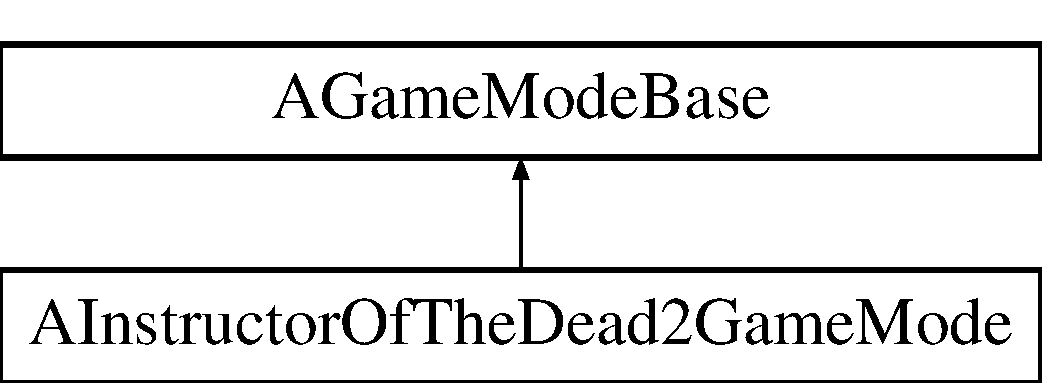
\includegraphics[height=2.000000cm]{class_a_instructor_of_the_dead2_game_mode}
\end{center}
\end{figure}


The documentation for this class was generated from the following files\+:\begin{DoxyCompactItemize}
\item 
Source/\+Instructor\+Of\+The\+Dead2/Instructor\+Of\+The\+Dead2\+Game\+Mode.\+h\item 
Source/\+Instructor\+Of\+The\+Dead2/Instructor\+Of\+The\+Dead2\+Game\+Mode.\+cpp\end{DoxyCompactItemize}

\hypertarget{class_a_level_boundary}{}\section{A\+Level\+Boundary Class Reference}
\label{class_a_level_boundary}\index{A\+Level\+Boundary@{A\+Level\+Boundary}}
Inheritance diagram for A\+Level\+Boundary\+:\begin{figure}[H]
\begin{center}
\leavevmode
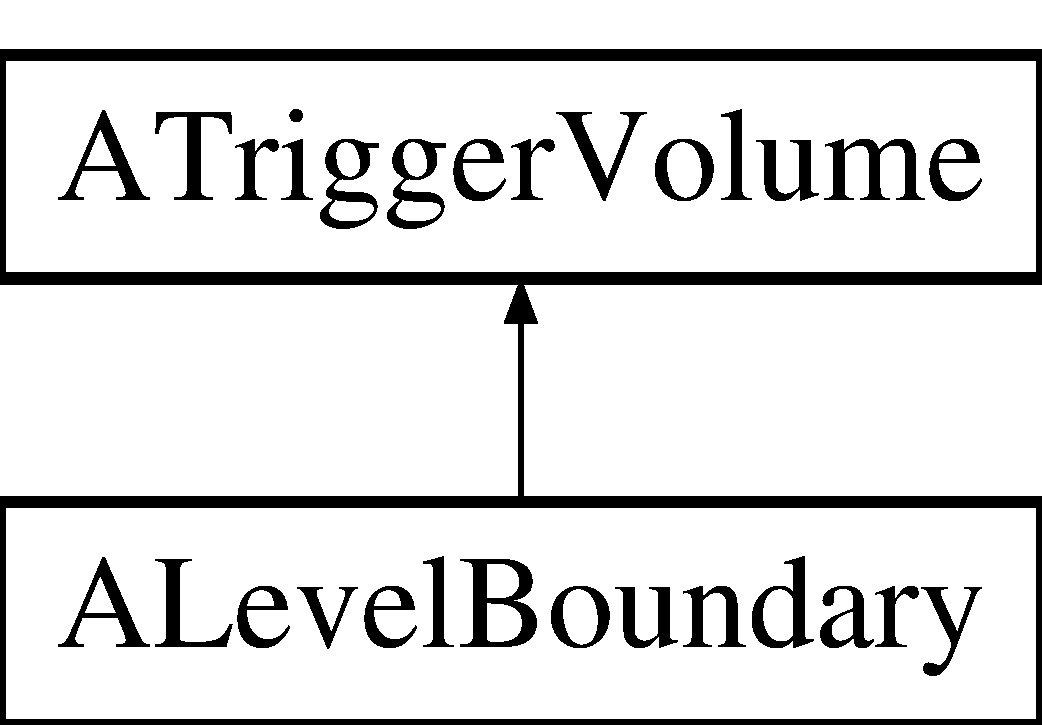
\includegraphics[height=2.000000cm]{class_a_level_boundary}
\end{center}
\end{figure}
\subsection*{Public Member Functions}
\begin{DoxyCompactItemize}
\item 
\mbox{\Hypertarget{class_a_level_boundary_af75a32e183b2fb04f37ef82596e7c812}\label{class_a_level_boundary_af75a32e183b2fb04f37ef82596e7c812}} 
void \mbox{\hyperlink{class_a_level_boundary_af75a32e183b2fb04f37ef82596e7c812}{On\+Overlap\+Begin}} (class A\+Actor $\ast$Overlapped\+Actor, class A\+Actor $\ast$Other\+Actor)
\begin{DoxyCompactList}\small\item\em Overriden Collisons Checking Method used to respawn a player if they went \char`\"{}out of bounds\char`\"{}. Called when the collsion begins. \end{DoxyCompactList}\item 
\mbox{\Hypertarget{class_a_level_boundary_a60671f338cc8ec077390965d975e0b20}\label{class_a_level_boundary_a60671f338cc8ec077390965d975e0b20}} 
void \mbox{\hyperlink{class_a_level_boundary_a60671f338cc8ec077390965d975e0b20}{On\+Overlap\+End}} (class A\+Actor $\ast$Overlapped\+Actor, class A\+Actor $\ast$Over\+Actor)
\begin{DoxyCompactList}\small\item\em Overriden Collisons Checking Method used to respawn a player if they went \char`\"{}out of bounds\char`\"{}. Called After the collision ends. \end{DoxyCompactList}\end{DoxyCompactItemize}
\subsection*{Public Attributes}
\begin{DoxyCompactItemize}
\item 
\mbox{\Hypertarget{class_a_level_boundary_a87be1c7307ff07bd9ad6cf5a51baa7b2}\label{class_a_level_boundary_a87be1c7307ff07bd9ad6cf5a51baa7b2}} 
F\+Vector \mbox{\hyperlink{class_a_level_boundary_a87be1c7307ff07bd9ad6cf5a51baa7b2}{Respawn}} = F\+Vector(700, 0, 8500)
\begin{DoxyCompactList}\small\item\em Respawn Location. \end{DoxyCompactList}\end{DoxyCompactItemize}
\subsection*{Protected Member Functions}
\begin{DoxyCompactItemize}
\item 
\mbox{\Hypertarget{class_a_level_boundary_aacde6fc2bd8835587d940b4b23871841}\label{class_a_level_boundary_aacde6fc2bd8835587d940b4b23871841}} 
virtual void \mbox{\hyperlink{class_a_level_boundary_aacde6fc2bd8835587d940b4b23871841}{Begin\+Play}} () override
\begin{DoxyCompactList}\small\item\em Callback Function. \end{DoxyCompactList}\end{DoxyCompactItemize}


The documentation for this class was generated from the following files\+:\begin{DoxyCompactItemize}
\item 
Source/\+Instructor\+Of\+The\+Dead2/\+Public/Level\+Boundary.\+h\item 
Source/\+Instructor\+Of\+The\+Dead2/\+Private/Level\+Boundary.\+cpp\end{DoxyCompactItemize}

\hypertarget{class_a_main_character}{}\section{A\+Main\+Character Class Reference}
\label{class_a_main_character}\index{A\+Main\+Character@{A\+Main\+Character}}
Inheritance diagram for A\+Main\+Character\+:\begin{figure}[H]
\begin{center}
\leavevmode
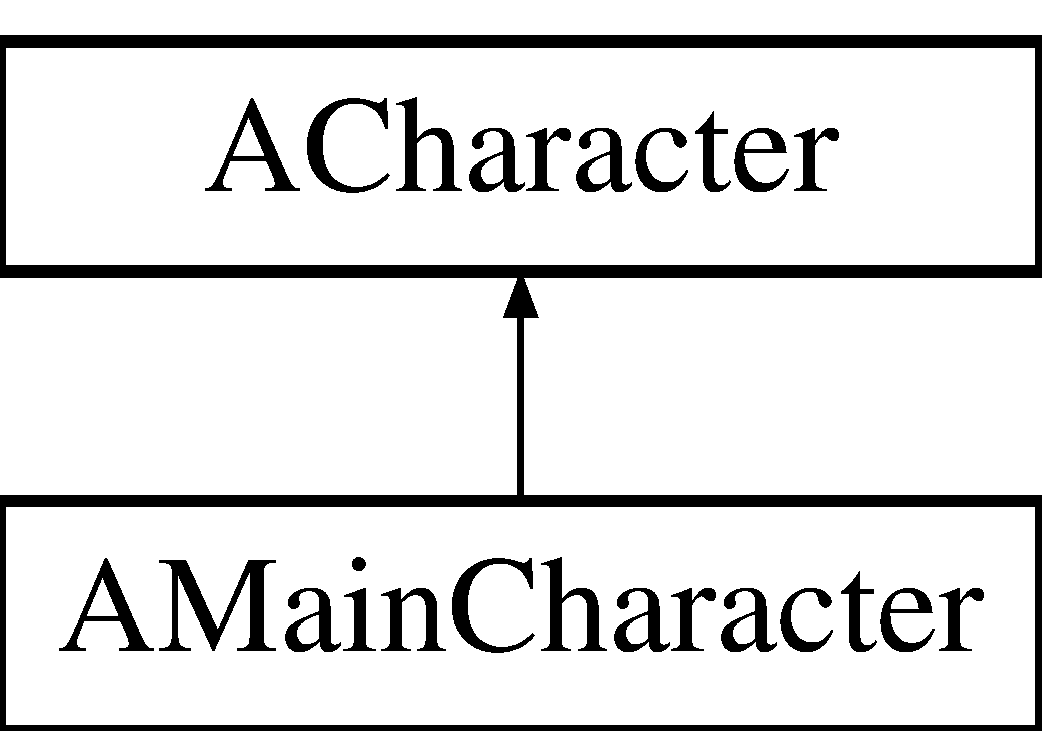
\includegraphics[height=2.000000cm]{class_a_main_character}
\end{center}
\end{figure}
\subsection*{Public Member Functions}
\begin{DoxyCompactItemize}
\item 
\mbox{\Hypertarget{class_a_main_character_a44a6be77fb1c8617c144a85fc084ad2b}\label{class_a_main_character_a44a6be77fb1c8617c144a85fc084ad2b}} 
virtual void {\bfseries Tick} (float Delta\+Time) override
\item 
\mbox{\Hypertarget{class_a_main_character_a96eb814e0d995ca16f33e92256756046}\label{class_a_main_character_a96eb814e0d995ca16f33e92256756046}} 
virtual void {\bfseries Setup\+Player\+Input\+Component} (class U\+Input\+Component $\ast$Player\+Input\+Component) override
\item 
\mbox{\Hypertarget{class_a_main_character_adb24c0fcbd3fe89d3b246981b16b8b5e}\label{class_a_main_character_adb24c0fcbd3fe89d3b246981b16b8b5e}} 
virtual F\+Vector {\bfseries Get\+Pawn\+View\+Location} () const override
\item 
\mbox{\Hypertarget{class_a_main_character_a2e3680c05b799891aa06311103314f40}\label{class_a_main_character_a2e3680c05b799891aa06311103314f40}} 
void {\bfseries Reset\+Fire} ()
\end{DoxyCompactItemize}
\subsection*{Public Attributes}
\begin{DoxyCompactItemize}
\item 
\mbox{\Hypertarget{class_a_main_character_a03aaa75e5621aece381717731ade0529}\label{class_a_main_character_a03aaa75e5621aece381717731ade0529}} 
bool {\bfseries player\+Can\+Fire}
\item 
\mbox{\Hypertarget{class_a_main_character_aeb723bc23c75b06e706ae1e973d6e14e}\label{class_a_main_character_aeb723bc23c75b06e706ae1e973d6e14e}} 
F\+Timer\+Handle {\bfseries Fire\+Delay}
\end{DoxyCompactItemize}
\subsection*{Protected Member Functions}
\begin{DoxyCompactItemize}
\item 
\mbox{\Hypertarget{class_a_main_character_a096ef46022cd84777b571482729ed02f}\label{class_a_main_character_a096ef46022cd84777b571482729ed02f}} 
virtual void {\bfseries Begin\+Play} () override
\item 
\mbox{\Hypertarget{class_a_main_character_aa85b946058cdc5f9b68ce529c9c680d8}\label{class_a_main_character_aa85b946058cdc5f9b68ce529c9c680d8}} 
void {\bfseries Move\+Forward} (float Value)
\item 
\mbox{\Hypertarget{class_a_main_character_aa3b2268816c54828d166ea626fdde411}\label{class_a_main_character_aa3b2268816c54828d166ea626fdde411}} 
void {\bfseries Move\+Right} (float Value)
\item 
\mbox{\Hypertarget{class_a_main_character_a44625f8c76490dfa989dc046b0612e07}\label{class_a_main_character_a44625f8c76490dfa989dc046b0612e07}} 
void {\bfseries Begin\+Crouch} ()
\item 
\mbox{\Hypertarget{class_a_main_character_a633a5955e941f4ff343709eed9141154}\label{class_a_main_character_a633a5955e941f4ff343709eed9141154}} 
void {\bfseries End\+Crouch} ()
\item 
\mbox{\Hypertarget{class_a_main_character_a4f7eea1e58e20b96564f3408f49737b6}\label{class_a_main_character_a4f7eea1e58e20b96564f3408f49737b6}} 
void {\bfseries Begin\+Zoom} ()
\item 
\mbox{\Hypertarget{class_a_main_character_ab226b5c0e4c8fa348e61f0da84680d3e}\label{class_a_main_character_ab226b5c0e4c8fa348e61f0da84680d3e}} 
void {\bfseries End\+Zoom} ()
\item 
\mbox{\Hypertarget{class_a_main_character_a741be0918633d2d40692e97dfba67d69}\label{class_a_main_character_a741be0918633d2d40692e97dfba67d69}} 
void {\bfseries Fire} ()
\end{DoxyCompactItemize}
\subsection*{Protected Attributes}
\begin{DoxyCompactItemize}
\item 
\mbox{\Hypertarget{class_a_main_character_a83ceb44c34596cf092b3fbdaf6d66649}\label{class_a_main_character_a83ceb44c34596cf092b3fbdaf6d66649}} 
U\+Camera\+Component $\ast$ {\bfseries Camera\+Comp}
\item 
\mbox{\Hypertarget{class_a_main_character_a149e14225fb4febe5e2dc1d2cdf976fc}\label{class_a_main_character_a149e14225fb4febe5e2dc1d2cdf976fc}} 
U\+Spring\+Arm\+Component $\ast$ {\bfseries Spring\+Arm\+Comp}
\item 
\mbox{\Hypertarget{class_a_main_character_a72af24b99adafa7b9d024732b00957c8}\label{class_a_main_character_a72af24b99adafa7b9d024732b00957c8}} 
bool {\bfseries b\+Wants\+To\+Zoom}
\item 
\mbox{\Hypertarget{class_a_main_character_a6be486b784b9900a9217a022be6bcaa2}\label{class_a_main_character_a6be486b784b9900a9217a022be6bcaa2}} 
float {\bfseries Zoomed\+F\+OV}
\item 
\mbox{\Hypertarget{class_a_main_character_acb71d1fee43be1c94560bc6f427bdc3f}\label{class_a_main_character_acb71d1fee43be1c94560bc6f427bdc3f}} 
float {\bfseries Zoom\+Interp\+Speed}
\item 
\mbox{\Hypertarget{class_a_main_character_aff0b6ec995a455073f0f4bb50cb15624}\label{class_a_main_character_aff0b6ec995a455073f0f4bb50cb15624}} 
float {\bfseries Default\+F\+OV}
\item 
\mbox{\Hypertarget{class_a_main_character_a564bee74c5e98baec0d48df92b73fd26}\label{class_a_main_character_a564bee74c5e98baec0d48df92b73fd26}} 
\mbox{\hyperlink{class_a_my_weapon___gun}{A\+My\+Weapon\+\_\+\+Gun}} $\ast$ {\bfseries Current\+Weapon}
\item 
\mbox{\Hypertarget{class_a_main_character_ab4701b65e5eaf3217ef385962c081620}\label{class_a_main_character_ab4701b65e5eaf3217ef385962c081620}} 
T\+Subclass\+Of$<$ \mbox{\hyperlink{class_a_my_weapon___gun}{A\+My\+Weapon\+\_\+\+Gun}} $>$ {\bfseries Starter\+Weapon\+Class}
\item 
\mbox{\Hypertarget{class_a_main_character_a661bb8f07ac38949071c5683b0d33251}\label{class_a_main_character_a661bb8f07ac38949071c5683b0d33251}} 
F\+Name {\bfseries Weapon\+Attach\+Socket\+Name}
\end{DoxyCompactItemize}


The documentation for this class was generated from the following files\+:\begin{DoxyCompactItemize}
\item 
Source/\+Instructor\+Of\+The\+Dead2/\+Public/Main\+Character.\+h\item 
Source/\+Instructor\+Of\+The\+Dead2/\+Private/Main\+Character.\+cpp\end{DoxyCompactItemize}

\hypertarget{class_a_my_weapon___gun}{}\section{A\+My\+Weapon\+\_\+\+Gun Class Reference}
\label{class_a_my_weapon___gun}\index{A\+My\+Weapon\+\_\+\+Gun@{A\+My\+Weapon\+\_\+\+Gun}}
Inheritance diagram for A\+My\+Weapon\+\_\+\+Gun\+:\begin{figure}[H]
\begin{center}
\leavevmode
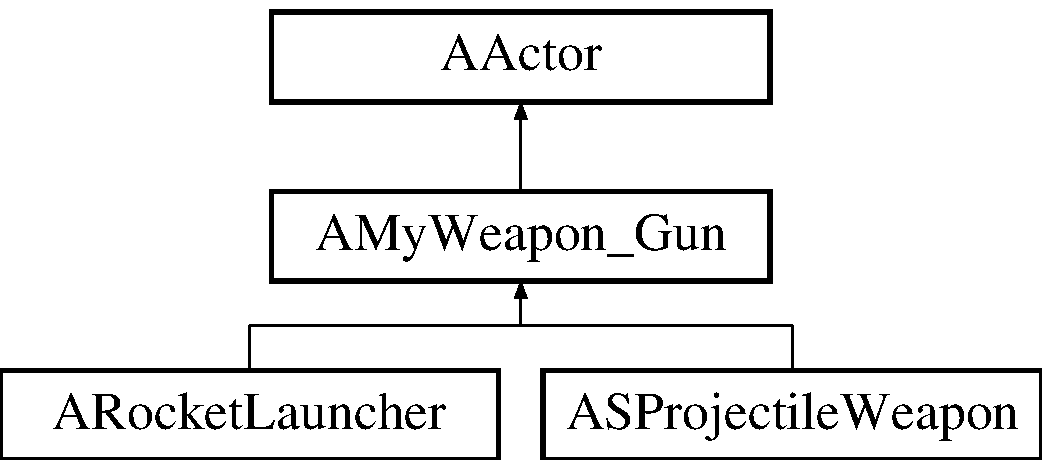
\includegraphics[height=3.000000cm]{class_a_my_weapon___gun}
\end{center}
\end{figure}
\subsection*{Public Member Functions}
\begin{DoxyCompactItemize}
\item 
virtual void \mbox{\hyperlink{class_a_my_weapon___gun_a8b430c2ea96f507fa29e2eceb7ebc552}{Fire}} ()
\end{DoxyCompactItemize}
\subsection*{Protected Member Functions}
\begin{DoxyCompactItemize}
\item 
void \mbox{\hyperlink{class_a_my_weapon___gun_a8d4f24314bfe7d7f722f1f03a9b52936}{Play\+Fire\+Effects}} (F\+Vector Trace\+End)
\item 
\mbox{\Hypertarget{class_a_my_weapon___gun_a705560269295e26bb47af646ddee16bb}\label{class_a_my_weapon___gun_a705560269295e26bb47af646ddee16bb}} 
void \mbox{\hyperlink{class_a_my_weapon___gun_a705560269295e26bb47af646ddee16bb}{Server\+Fire}} ()
\begin{DoxyCompactList}\small\item\em Has a player \char`\"{}fire\char`\"{} from the server\textquotesingle{}s end and then replicate the action. \end{DoxyCompactList}\item 
\mbox{\Hypertarget{class_a_my_weapon___gun_af37b774edf0e46530795e38cb55c69ae}\label{class_a_my_weapon___gun_af37b774edf0e46530795e38cb55c69ae}} 
void \mbox{\hyperlink{class_a_my_weapon___gun_af37b774edf0e46530795e38cb55c69ae}{On\+\_\+\+Rep\+\_\+\+Hit\+Scan\+Trace}} ()
\begin{DoxyCompactList}\small\item\em Sets \mbox{\hyperlink{class_a_my_weapon___gun_a63a32b90438b170a8b5b41a83051cb3e}{Hit\+Scan\+Trace()}} to replicate. \end{DoxyCompactList}\item 
void \mbox{\hyperlink{class_a_my_weapon___gun_a2a734edf94e9c1aa40194c60a6116c99}{Play\+Impact\+Effects}} (E\+Physical\+Surface Surface\+Type, F\+Vector Impact\+Point)
\end{DoxyCompactItemize}
\subsection*{Protected Attributes}
\begin{DoxyCompactItemize}
\item 
\mbox{\Hypertarget{class_a_my_weapon___gun_ae5cc40d0c60ca3a5120acf10a1b1f4c7}\label{class_a_my_weapon___gun_ae5cc40d0c60ca3a5120acf10a1b1f4c7}} 
U\+Skeletal\+Mesh\+Component $\ast$ \mbox{\hyperlink{class_a_my_weapon___gun_ae5cc40d0c60ca3a5120acf10a1b1f4c7}{Mesh\+Comp}}
\begin{DoxyCompactList}\small\item\em Pointer to wireframe. Used for skinning. \end{DoxyCompactList}\item 
\mbox{\Hypertarget{class_a_my_weapon___gun_a8d5171dbf961d142e836c08c61042fd1}\label{class_a_my_weapon___gun_a8d5171dbf961d142e836c08c61042fd1}} 
T\+Subclass\+Of$<$ U\+Damage\+Type $>$ \mbox{\hyperlink{class_a_my_weapon___gun_a8d5171dbf961d142e836c08c61042fd1}{Damage\+Type}}
\begin{DoxyCompactList}\small\item\em Determines the damage type. \end{DoxyCompactList}\item 
\mbox{\Hypertarget{class_a_my_weapon___gun_a3be0763373c47e77d857658ad55a78b9}\label{class_a_my_weapon___gun_a3be0763373c47e77d857658ad55a78b9}} 
F\+Name \mbox{\hyperlink{class_a_my_weapon___gun_a3be0763373c47e77d857658ad55a78b9}{Muzzle\+Socket\+Name}}
\begin{DoxyCompactList}\small\item\em Reference to the endpoint of the gun object. \end{DoxyCompactList}\item 
\mbox{\Hypertarget{class_a_my_weapon___gun_a8c55f6a25191a005d54c60ab9fe2c416}\label{class_a_my_weapon___gun_a8c55f6a25191a005d54c60ab9fe2c416}} 
F\+Name \mbox{\hyperlink{class_a_my_weapon___gun_a8c55f6a25191a005d54c60ab9fe2c416}{Tracer\+Target\+Name}}
\begin{DoxyCompactList}\small\item\em Reference to the tracer object. \end{DoxyCompactList}\item 
\mbox{\Hypertarget{class_a_my_weapon___gun_a679469b189976f66e5c55f9fdeccb885}\label{class_a_my_weapon___gun_a679469b189976f66e5c55f9fdeccb885}} 
U\+Particle\+System $\ast$ \mbox{\hyperlink{class_a_my_weapon___gun_a679469b189976f66e5c55f9fdeccb885}{Muzzle\+Effect}}
\begin{DoxyCompactList}\small\item\em Handles Particle Effects for the gun\textquotesingle{}s muzzle. \end{DoxyCompactList}\item 
\mbox{\Hypertarget{class_a_my_weapon___gun_ac2f8ae09bfe4a45ffecd1152992b7bd1}\label{class_a_my_weapon___gun_ac2f8ae09bfe4a45ffecd1152992b7bd1}} 
U\+Particle\+System $\ast$ \mbox{\hyperlink{class_a_my_weapon___gun_ac2f8ae09bfe4a45ffecd1152992b7bd1}{Default\+Impact\+Effect}}
\begin{DoxyCompactList}\small\item\em Handles default particle effect for when a projectile imapcts an object. \end{DoxyCompactList}\item 
\mbox{\Hypertarget{class_a_my_weapon___gun_a54d0bc79091a1c6c1ff1024a504a913e}\label{class_a_my_weapon___gun_a54d0bc79091a1c6c1ff1024a504a913e}} 
U\+Particle\+System $\ast$ \mbox{\hyperlink{class_a_my_weapon___gun_a54d0bc79091a1c6c1ff1024a504a913e}{Flesh\+Impact\+Effects}}
\begin{DoxyCompactList}\small\item\em Handles default particle effect for when a projectile impacts a a player. \end{DoxyCompactList}\item 
\mbox{\Hypertarget{class_a_my_weapon___gun_a14dd5df426696f79aa347bb870e55a8a}\label{class_a_my_weapon___gun_a14dd5df426696f79aa347bb870e55a8a}} 
U\+Particle\+System $\ast$ \mbox{\hyperlink{class_a_my_weapon___gun_a14dd5df426696f79aa347bb870e55a8a}{Tracer\+Effect}}
\begin{DoxyCompactList}\small\item\em Handles the particle effect for creating the \char`\"{}tracer\char`\"{} vector. \end{DoxyCompactList}\item 
\mbox{\Hypertarget{class_a_my_weapon___gun_ac88147e1d8d4c2e0fcc4b99508151d95}\label{class_a_my_weapon___gun_ac88147e1d8d4c2e0fcc4b99508151d95}} 
T\+Subclass\+Of$<$ U\+Camera\+Shake $>$ \mbox{\hyperlink{class_a_my_weapon___gun_ac88147e1d8d4c2e0fcc4b99508151d95}{Fire\+Cam\+Shake}}
\begin{DoxyCompactList}\small\item\em Shakes the camera when a gun is fired. \end{DoxyCompactList}\item 
\mbox{\Hypertarget{class_a_my_weapon___gun_a249e1fd79607e29492373ec47fdea572}\label{class_a_my_weapon___gun_a249e1fd79607e29492373ec47fdea572}} 
float \mbox{\hyperlink{class_a_my_weapon___gun_a249e1fd79607e29492373ec47fdea572}{Base\+Damage}}
\begin{DoxyCompactList}\small\item\em The default damage amount. \end{DoxyCompactList}\item 
\mbox{\Hypertarget{class_a_my_weapon___gun_a63a32b90438b170a8b5b41a83051cb3e}\label{class_a_my_weapon___gun_a63a32b90438b170a8b5b41a83051cb3e}} 
\mbox{\hyperlink{struct_f_hit_scan_trace}{F\+Hit\+Scan\+Trace}} \mbox{\hyperlink{class_a_my_weapon___gun_a63a32b90438b170a8b5b41a83051cb3e}{Hit\+Scan\+Trace}}
\begin{DoxyCompactList}\small\item\em Stores the. \end{DoxyCompactList}\end{DoxyCompactItemize}


\subsection{Member Function Documentation}
\mbox{\Hypertarget{class_a_my_weapon___gun_a8b430c2ea96f507fa29e2eceb7ebc552}\label{class_a_my_weapon___gun_a8b430c2ea96f507fa29e2eceb7ebc552}} 
\index{A\+My\+Weapon\+\_\+\+Gun@{A\+My\+Weapon\+\_\+\+Gun}!Fire@{Fire}}
\index{Fire@{Fire}!A\+My\+Weapon\+\_\+\+Gun@{A\+My\+Weapon\+\_\+\+Gun}}
\subsubsection{\texorpdfstring{Fire()}{Fire()}}
{\footnotesize\ttfamily void A\+My\+Weapon\+\_\+\+Gun\+::\+Fire (\begin{DoxyParamCaption}{ }\end{DoxyParamCaption})\hspace{0.3cm}{\ttfamily [virtual]}}

Fires the gun. Short circuits, if called on a client, and serverfire() is called instead. 

Reimplemented in \mbox{\hyperlink{class_a_rocket_launcher_a32f4db5a70f3a9e6b8cf0d8c0e84f78b}{A\+Rocket\+Launcher}}.

\mbox{\Hypertarget{class_a_my_weapon___gun_a8d4f24314bfe7d7f722f1f03a9b52936}\label{class_a_my_weapon___gun_a8d4f24314bfe7d7f722f1f03a9b52936}} 
\index{A\+My\+Weapon\+\_\+\+Gun@{A\+My\+Weapon\+\_\+\+Gun}!Play\+Fire\+Effects@{Play\+Fire\+Effects}}
\index{Play\+Fire\+Effects@{Play\+Fire\+Effects}!A\+My\+Weapon\+\_\+\+Gun@{A\+My\+Weapon\+\_\+\+Gun}}
\subsubsection{\texorpdfstring{Play\+Fire\+Effects()}{PlayFireEffects()}}
{\footnotesize\ttfamily void A\+My\+Weapon\+\_\+\+Gun\+::\+Play\+Fire\+Effects (\begin{DoxyParamCaption}\item[{F\+Vector}]{Trace\+End }\end{DoxyParamCaption})\hspace{0.3cm}{\ttfamily [protected]}}

Generates a Fire Effect based on muzzle and tracer effects.


\begin{DoxyParams}{Parameters}
{\em Trace\+End} & Used to draw the tracer effect if used \\
\hline
\end{DoxyParams}
\mbox{\Hypertarget{class_a_my_weapon___gun_a2a734edf94e9c1aa40194c60a6116c99}\label{class_a_my_weapon___gun_a2a734edf94e9c1aa40194c60a6116c99}} 
\index{A\+My\+Weapon\+\_\+\+Gun@{A\+My\+Weapon\+\_\+\+Gun}!Play\+Impact\+Effects@{Play\+Impact\+Effects}}
\index{Play\+Impact\+Effects@{Play\+Impact\+Effects}!A\+My\+Weapon\+\_\+\+Gun@{A\+My\+Weapon\+\_\+\+Gun}}
\subsubsection{\texorpdfstring{Play\+Impact\+Effects()}{PlayImpactEffects()}}
{\footnotesize\ttfamily void A\+My\+Weapon\+\_\+\+Gun\+::\+Play\+Impact\+Effects (\begin{DoxyParamCaption}\item[{E\+Physical\+Surface}]{Surface\+Type,  }\item[{F\+Vector}]{Impact\+Point }\end{DoxyParamCaption})\hspace{0.3cm}{\ttfamily [protected]}}

Generates a Impact Effect based on the Surfacetype hit.


\begin{DoxyParams}{Parameters}
{\em Surface\+Type} & Indicates whether the surface is a player or non-\/player object \\
\hline
{\em Impact\+Point} & The location where the projectile hit \\
\hline
\end{DoxyParams}


The documentation for this class was generated from the following files\+:\begin{DoxyCompactItemize}
\item 
Source/\+Instructor\+Of\+The\+Dead2/My\+Weapon\+\_\+\+Gun.\+h\item 
Source/\+Instructor\+Of\+The\+Dead2/My\+Weapon\+\_\+\+Gun.\+cpp\end{DoxyCompactItemize}

\hypertarget{class_a_rocket_launcher}{}\section{A\+Rocket\+Launcher Class Reference}
\label{class_a_rocket_launcher}\index{A\+Rocket\+Launcher@{A\+Rocket\+Launcher}}
Inheritance diagram for A\+Rocket\+Launcher\+:\begin{figure}[H]
\begin{center}
\leavevmode
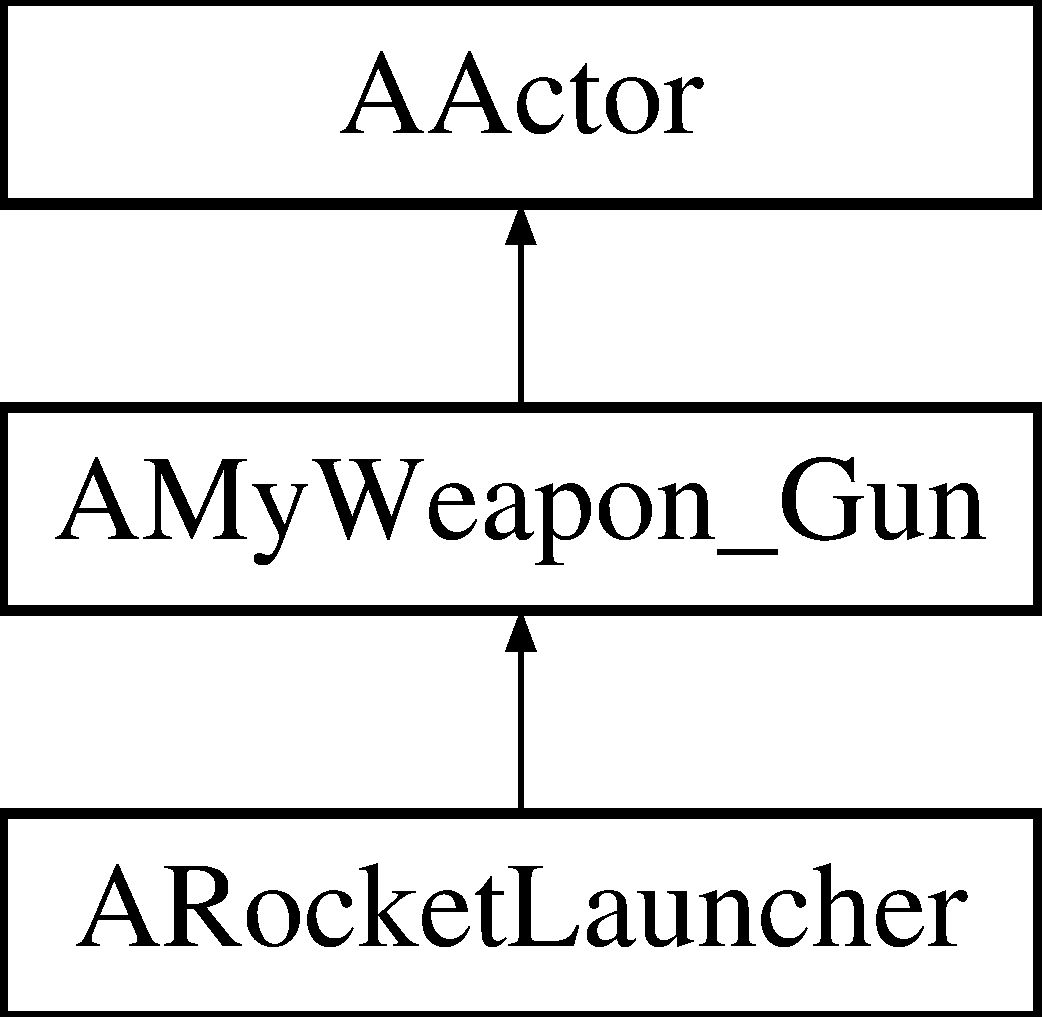
\includegraphics[height=3.000000cm]{class_a_rocket_launcher}
\end{center}
\end{figure}
\subsection*{Public Member Functions}
\begin{DoxyCompactItemize}
\item 
virtual void \mbox{\hyperlink{class_a_rocket_launcher_a32f4db5a70f3a9e6b8cf0d8c0e84f78b}{Fire}} () override
\item 
\mbox{\Hypertarget{class_a_rocket_launcher_af09c3d3fd27a768ddafde48045b3e4e5}\label{class_a_rocket_launcher_af09c3d3fd27a768ddafde48045b3e4e5}} 
void {\bfseries Server\+Fire} ()
\end{DoxyCompactItemize}
\subsection*{Public Attributes}
\begin{DoxyCompactItemize}
\item 
\mbox{\Hypertarget{class_a_rocket_launcher_a4974bb444bf93eb2c6d7d6e04e6ea4a0}\label{class_a_rocket_launcher_a4974bb444bf93eb2c6d7d6e04e6ea4a0}} 
T\+Subclass\+Of$<$ A\+Actor $>$ {\bfseries Rocket\+Launcher\+Class}
\end{DoxyCompactItemize}
\subsection*{Additional Inherited Members}


\subsection{Member Function Documentation}
\mbox{\Hypertarget{class_a_rocket_launcher_a32f4db5a70f3a9e6b8cf0d8c0e84f78b}\label{class_a_rocket_launcher_a32f4db5a70f3a9e6b8cf0d8c0e84f78b}} 
\index{A\+Rocket\+Launcher@{A\+Rocket\+Launcher}!Fire@{Fire}}
\index{Fire@{Fire}!A\+Rocket\+Launcher@{A\+Rocket\+Launcher}}
\subsubsection{\texorpdfstring{Fire()}{Fire()}}
{\footnotesize\ttfamily void A\+Rocket\+Launcher\+::\+Fire (\begin{DoxyParamCaption}{ }\end{DoxyParamCaption})\hspace{0.3cm}{\ttfamily [override]}, {\ttfamily [virtual]}}

Fires the gun. Short circuits, if called on a client, and serverfire() is called instead. 

Reimplemented from \mbox{\hyperlink{class_a_my_weapon___gun_a8b430c2ea96f507fa29e2eceb7ebc552}{A\+My\+Weapon\+\_\+\+Gun}}.



The documentation for this class was generated from the following files\+:\begin{DoxyCompactItemize}
\item 
Source/\+Instructor\+Of\+The\+Dead2/\+Public/Rocket\+Launcher.\+h\item 
Source/\+Instructor\+Of\+The\+Dead2/\+Private/Rocket\+Launcher.\+cpp\end{DoxyCompactItemize}

\hypertarget{class_a_s_projectile_weapon}{}\section{A\+S\+Projectile\+Weapon Class Reference}
\label{class_a_s_projectile_weapon}\index{A\+S\+Projectile\+Weapon@{A\+S\+Projectile\+Weapon}}
Inheritance diagram for A\+S\+Projectile\+Weapon\+:\begin{figure}[H]
\begin{center}
\leavevmode
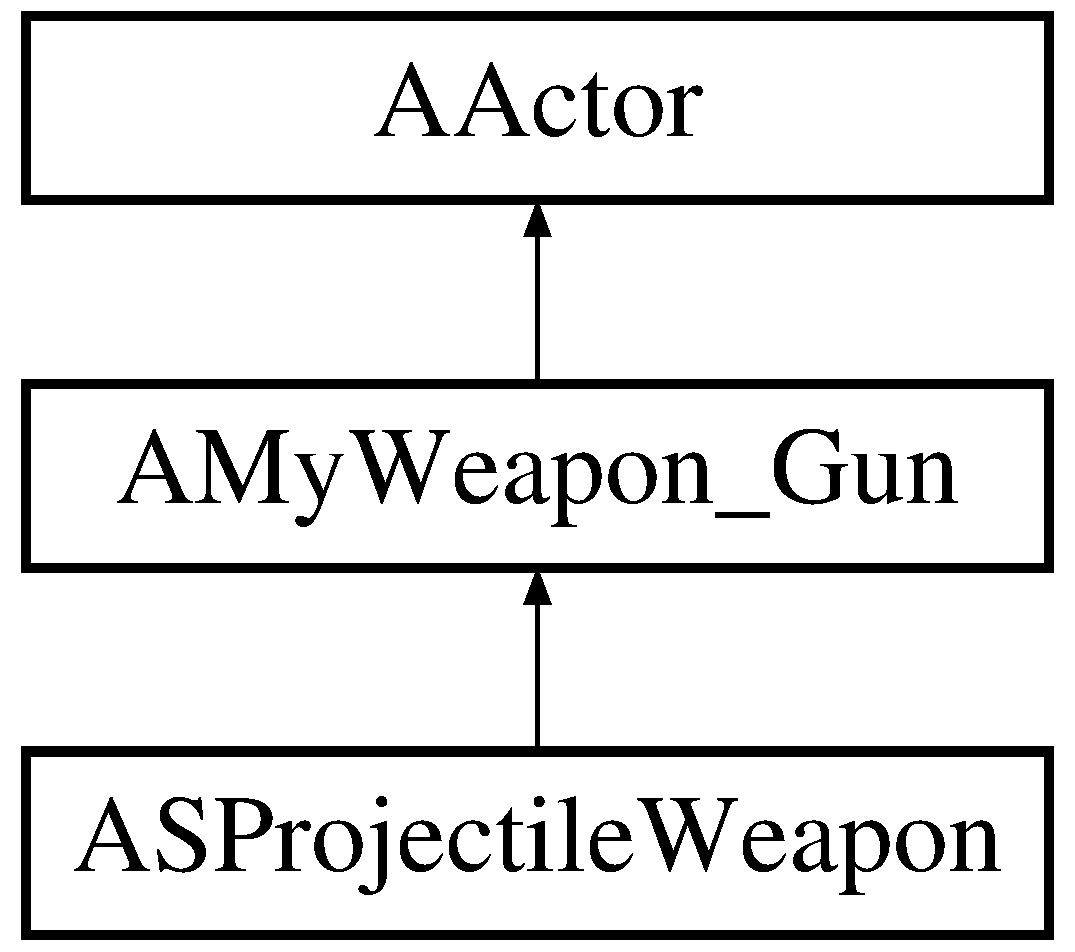
\includegraphics[height=3.000000cm]{class_a_s_projectile_weapon}
\end{center}
\end{figure}
\subsection*{Additional Inherited Members}


The documentation for this class was generated from the following file\+:\begin{DoxyCompactItemize}
\item 
Source/\+Instructor\+Of\+The\+Dead2/\+Public/S\+Projectile\+Weapon.\+h\end{DoxyCompactItemize}

\hypertarget{struct_f_hit_scan_trace}{}\section{F\+Hit\+Scan\+Trace Struct Reference}
\label{struct_f_hit_scan_trace}\index{F\+Hit\+Scan\+Trace@{F\+Hit\+Scan\+Trace}}
\subsection*{Public Attributes}
\begin{DoxyCompactItemize}
\item 
\mbox{\Hypertarget{struct_f_hit_scan_trace_adf2be583210a6d43ee5697cff3c46040}\label{struct_f_hit_scan_trace_adf2be583210a6d43ee5697cff3c46040}} 
T\+Enum\+As\+Byte$<$ E\+Physical\+Surface $>$ \mbox{\hyperlink{struct_f_hit_scan_trace_adf2be583210a6d43ee5697cff3c46040}{Surface\+Type}}
\begin{DoxyCompactList}\small\item\em Determines whether the target is a player or non-\/player object. \end{DoxyCompactList}\item 
\mbox{\Hypertarget{struct_f_hit_scan_trace_a603adcd1a2ce6f1c504ee112a0978d5a}\label{struct_f_hit_scan_trace_a603adcd1a2ce6f1c504ee112a0978d5a}} 
F\+Vector\+\_\+\+Net\+Quantize \mbox{\hyperlink{struct_f_hit_scan_trace_a603adcd1a2ce6f1c504ee112a0978d5a}{Trace\+To}}
\begin{DoxyCompactList}\small\item\em Vector that the projectile follows. \end{DoxyCompactList}\end{DoxyCompactItemize}


The documentation for this struct was generated from the following file\+:\begin{DoxyCompactItemize}
\item 
Source/\+Instructor\+Of\+The\+Dead2/My\+Weapon\+\_\+\+Gun.\+h\end{DoxyCompactItemize}

\hypertarget{class_f_testing_module}{}\section{F\+Testing\+Module Class Reference}
\label{class_f_testing_module}\index{F\+Testing\+Module@{F\+Testing\+Module}}
Inheritance diagram for F\+Testing\+Module\+:\begin{figure}[H]
\begin{center}
\leavevmode
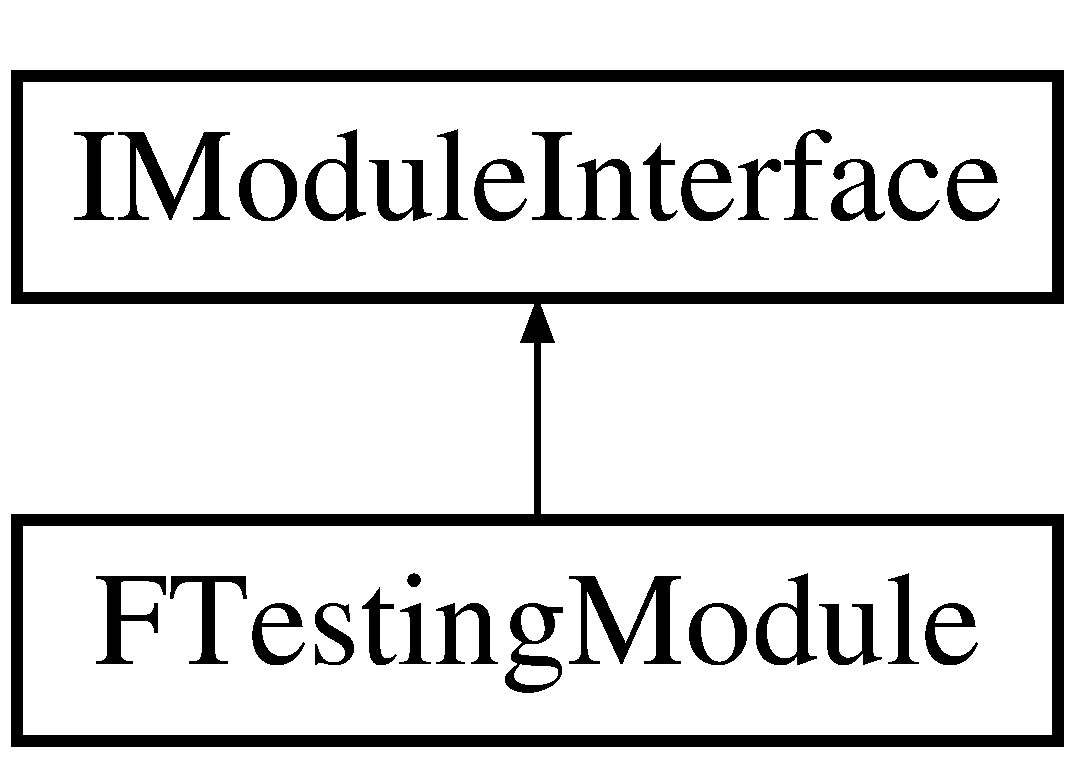
\includegraphics[height=2.000000cm]{class_f_testing_module}
\end{center}
\end{figure}
\subsection*{Public Member Functions}
\begin{DoxyCompactItemize}
\item 
\mbox{\Hypertarget{class_f_testing_module_a0d4c4e00c59e49db76da01eb960966f1}\label{class_f_testing_module_a0d4c4e00c59e49db76da01eb960966f1}} 
virtual void \mbox{\hyperlink{class_f_testing_module_a0d4c4e00c59e49db76da01eb960966f1}{Startup\+Module}} () override
\begin{DoxyCompactList}\small\item\em Setup Function. Logs startup. \end{DoxyCompactList}\item 
\mbox{\Hypertarget{class_f_testing_module_afac07308b91f8a5d54a7934b055a2030}\label{class_f_testing_module_afac07308b91f8a5d54a7934b055a2030}} 
virtual void \mbox{\hyperlink{class_f_testing_module_afac07308b91f8a5d54a7934b055a2030}{Shutdown\+Module}} () override
\begin{DoxyCompactList}\small\item\em Teardown Function. Logs shutdown. \end{DoxyCompactList}\end{DoxyCompactItemize}


The documentation for this class was generated from the following files\+:\begin{DoxyCompactItemize}
\item 
Source/\+Testing\+Module/\+Public/Testing\+Module.\+h\item 
Source/\+Testing\+Module/\+Private/Testing\+Module.\+cpp\end{DoxyCompactItemize}

\hypertarget{class_instructor_of_the_dead2}{}\section{Instructor\+Of\+The\+Dead2 Class Reference}
\label{class_instructor_of_the_dead2}\index{Instructor\+Of\+The\+Dead2@{Instructor\+Of\+The\+Dead2}}
Inheritance diagram for Instructor\+Of\+The\+Dead2\+:\begin{figure}[H]
\begin{center}
\leavevmode
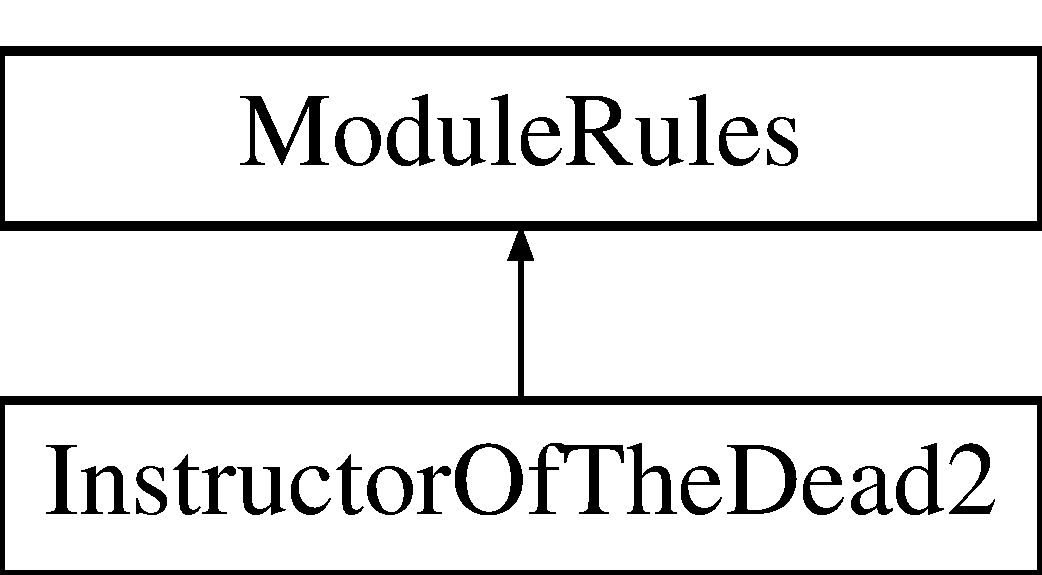
\includegraphics[height=2.000000cm]{class_instructor_of_the_dead2}
\end{center}
\end{figure}
\subsection*{Public Member Functions}
\begin{DoxyCompactItemize}
\item 
\mbox{\Hypertarget{class_instructor_of_the_dead2_a1be84c5444e47351a8f28a62159b500f}\label{class_instructor_of_the_dead2_a1be84c5444e47351a8f28a62159b500f}} 
{\bfseries Instructor\+Of\+The\+Dead2} (Read\+Only\+Target\+Rules Target)
\end{DoxyCompactItemize}


The documentation for this class was generated from the following file\+:\begin{DoxyCompactItemize}
\item 
Source/\+Instructor\+Of\+The\+Dead2/Instructor\+Of\+The\+Dead2.\+Build.\+cs\end{DoxyCompactItemize}

\hypertarget{class_instructor_of_the_dead2_editor_target}{}\section{Instructor\+Of\+The\+Dead2\+Editor\+Target Class Reference}
\label{class_instructor_of_the_dead2_editor_target}\index{Instructor\+Of\+The\+Dead2\+Editor\+Target@{Instructor\+Of\+The\+Dead2\+Editor\+Target}}
Inheritance diagram for Instructor\+Of\+The\+Dead2\+Editor\+Target\+:\begin{figure}[H]
\begin{center}
\leavevmode
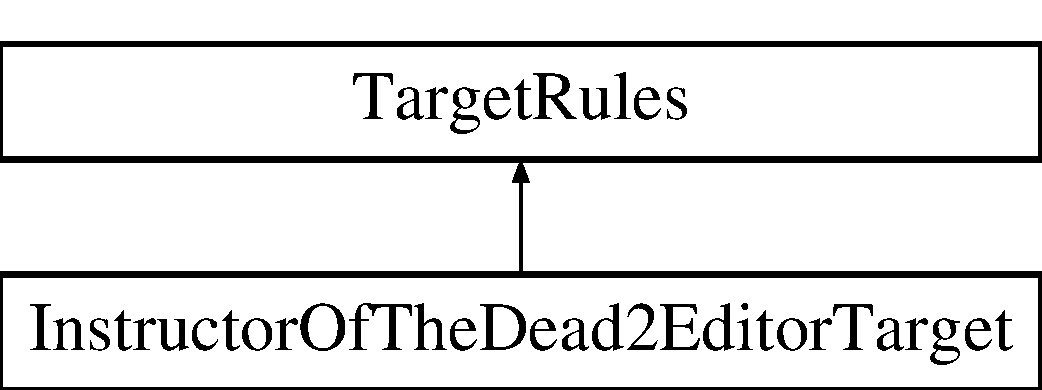
\includegraphics[height=2.000000cm]{class_instructor_of_the_dead2_editor_target}
\end{center}
\end{figure}
\subsection*{Public Member Functions}
\begin{DoxyCompactItemize}
\item 
\mbox{\Hypertarget{class_instructor_of_the_dead2_editor_target_a9572722a42cc5e7057e9e3ba5019c912}\label{class_instructor_of_the_dead2_editor_target_a9572722a42cc5e7057e9e3ba5019c912}} 
{\bfseries Instructor\+Of\+The\+Dead2\+Editor\+Target} (Target\+Info Target)
\end{DoxyCompactItemize}


The documentation for this class was generated from the following file\+:\begin{DoxyCompactItemize}
\item 
Source/Instructor\+Of\+The\+Dead2\+Editor.\+Target.\+cs\end{DoxyCompactItemize}

\hypertarget{class_instructor_of_the_dead2_target}{}\section{Instructor\+Of\+The\+Dead2\+Target Class Reference}
\label{class_instructor_of_the_dead2_target}\index{Instructor\+Of\+The\+Dead2\+Target@{Instructor\+Of\+The\+Dead2\+Target}}
Inheritance diagram for Instructor\+Of\+The\+Dead2\+Target\+:\begin{figure}[H]
\begin{center}
\leavevmode
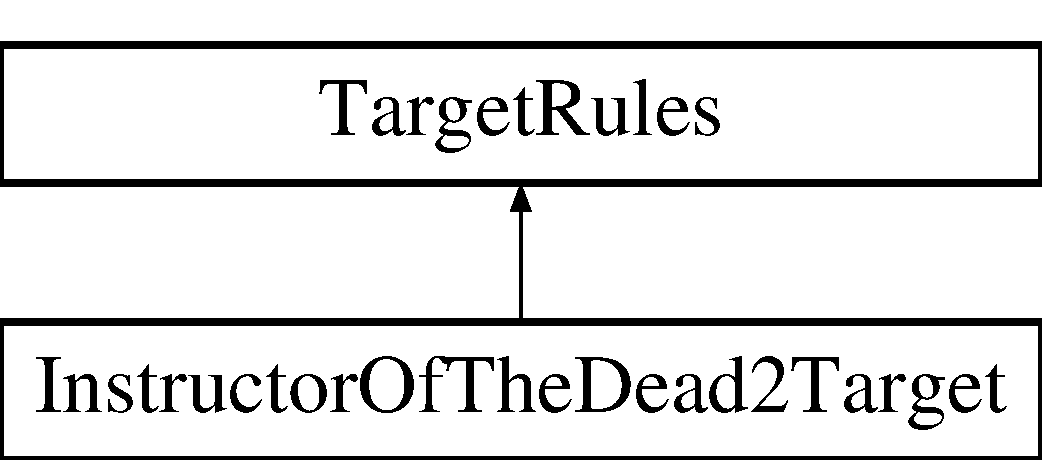
\includegraphics[height=2.000000cm]{class_instructor_of_the_dead2_target}
\end{center}
\end{figure}
\subsection*{Public Member Functions}
\begin{DoxyCompactItemize}
\item 
\mbox{\Hypertarget{class_instructor_of_the_dead2_target_a3be2fedb24e2765cb7f9bee24a5231ff}\label{class_instructor_of_the_dead2_target_a3be2fedb24e2765cb7f9bee24a5231ff}} 
{\bfseries Instructor\+Of\+The\+Dead2\+Target} (Target\+Info Target)
\end{DoxyCompactItemize}


The documentation for this class was generated from the following file\+:\begin{DoxyCompactItemize}
\item 
Source/Instructor\+Of\+The\+Dead2.\+Target.\+cs\end{DoxyCompactItemize}

\hypertarget{class_level_boundary_test}{}\section{Level\+Boundary\+Test Class Reference}
\label{class_level_boundary_test}\index{Level\+Boundary\+Test@{Level\+Boundary\+Test}}


The documentation for this class was generated from the following file\+:\begin{DoxyCompactItemize}
\item 
Source/\+Testing\+Module/\+Public/Level\+Boundary\+Test.\+h\end{DoxyCompactItemize}

\hypertarget{class_level_boundary_test2}{}\section{Level\+Boundary\+Test2 Class Reference}
\label{class_level_boundary_test2}\index{Level\+Boundary\+Test2@{Level\+Boundary\+Test2}}


The documentation for this class was generated from the following file\+:\begin{DoxyCompactItemize}
\item 
Source/\+Testing\+Module/\+Public/Level\+Boundary\+Test2.\+h\end{DoxyCompactItemize}

\hypertarget{class_my_health_component_testing}{}\section{My\+Health\+Component\+Testing Class Reference}
\label{class_my_health_component_testing}\index{My\+Health\+Component\+Testing@{My\+Health\+Component\+Testing}}


The documentation for this class was generated from the following file\+:\begin{DoxyCompactItemize}
\item 
Source/\+Testing\+Module/\+Public/My\+Health\+Component\+Testing.\+h\end{DoxyCompactItemize}

\hypertarget{class_my_weapon___gun_test1}{}\section{My\+Weapon\+\_\+\+Gun\+Test1 Class Reference}
\label{class_my_weapon___gun_test1}\index{My\+Weapon\+\_\+\+Gun\+Test1@{My\+Weapon\+\_\+\+Gun\+Test1}}


The documentation for this class was generated from the following file\+:\begin{DoxyCompactItemize}
\item 
Source/\+Testing\+Module/\+Public/My\+Weapon\+\_\+\+Gun\+Test1.\+h\end{DoxyCompactItemize}

\hypertarget{class_my_weapon___gun_test2}{}\section{My\+Weapon\+\_\+\+Gun\+Test2 Class Reference}
\label{class_my_weapon___gun_test2}\index{My\+Weapon\+\_\+\+Gun\+Test2@{My\+Weapon\+\_\+\+Gun\+Test2}}


The documentation for this class was generated from the following file\+:\begin{DoxyCompactItemize}
\item 
Source/\+Testing\+Module/\+Public/My\+Weapon\+\_\+\+Gun\+Test2.\+h\end{DoxyCompactItemize}

\hypertarget{class_my_weapon___gun_test3}{}\section{My\+Weapon\+\_\+\+Gun\+Test3 Class Reference}
\label{class_my_weapon___gun_test3}\index{My\+Weapon\+\_\+\+Gun\+Test3@{My\+Weapon\+\_\+\+Gun\+Test3}}


The documentation for this class was generated from the following file\+:\begin{DoxyCompactItemize}
\item 
Source/\+Testing\+Module/\+Public/My\+Weapon\+\_\+\+Gun\+Test3.\+h\end{DoxyCompactItemize}

\hypertarget{class_my_weapon___gun_test4}{}\section{My\+Weapon\+\_\+\+Gun\+Test4 Class Reference}
\label{class_my_weapon___gun_test4}\index{My\+Weapon\+\_\+\+Gun\+Test4@{My\+Weapon\+\_\+\+Gun\+Test4}}


The documentation for this class was generated from the following file\+:\begin{DoxyCompactItemize}
\item 
Source/\+Testing\+Module/\+Public/My\+Weapon\+\_\+\+Gun\+Test4.\+h\end{DoxyCompactItemize}

\hypertarget{class_my_weapon___gun_test5}{}\section{My\+Weapon\+\_\+\+Gun\+Test5 Class Reference}
\label{class_my_weapon___gun_test5}\index{My\+Weapon\+\_\+\+Gun\+Test5@{My\+Weapon\+\_\+\+Gun\+Test5}}


The documentation for this class was generated from the following file\+:\begin{DoxyCompactItemize}
\item 
Source/\+Testing\+Module/\+Public/My\+Weapon\+\_\+\+Gun\+Test5.\+h\end{DoxyCompactItemize}

\hypertarget{class_rocket_launcher_test}{}\section{Rocket\+Launcher\+Test Class Reference}
\label{class_rocket_launcher_test}\index{Rocket\+Launcher\+Test@{Rocket\+Launcher\+Test}}


The documentation for this class was generated from the following file\+:\begin{DoxyCompactItemize}
\item 
Source/\+Testing\+Module/\+Public/Rocket\+Launcher\+Test.\+h\end{DoxyCompactItemize}

\hypertarget{class_rocket_launcher_test2}{}\section{Rocket\+Launcher\+Test2 Class Reference}
\label{class_rocket_launcher_test2}\index{Rocket\+Launcher\+Test2@{Rocket\+Launcher\+Test2}}


The documentation for this class was generated from the following file\+:\begin{DoxyCompactItemize}
\item 
Source/\+Testing\+Module/\+Public/Rocket\+Launcher\+Test2.\+h\end{DoxyCompactItemize}

\hypertarget{class_rocket_launcher_test3}{}\section{Rocket\+Launcher\+Test3 Class Reference}
\label{class_rocket_launcher_test3}\index{Rocket\+Launcher\+Test3@{Rocket\+Launcher\+Test3}}


The documentation for this class was generated from the following file\+:\begin{DoxyCompactItemize}
\item 
Source/\+Testing\+Module/\+Public/Rocket\+Launcher\+Test3.\+h\end{DoxyCompactItemize}

\hypertarget{class_rocket_launcher_test4}{}\section{Rocket\+Launcher\+Test4 Class Reference}
\label{class_rocket_launcher_test4}\index{Rocket\+Launcher\+Test4@{Rocket\+Launcher\+Test4}}


The documentation for this class was generated from the following file\+:\begin{DoxyCompactItemize}
\item 
Source/\+Testing\+Module/\+Public/Rocket\+Launcher\+Test4.\+h\end{DoxyCompactItemize}

\hypertarget{class_steam_test}{}\section{Steam\+Test Class Reference}
\label{class_steam_test}\index{Steam\+Test@{Steam\+Test}}


The documentation for this class was generated from the following file\+:\begin{DoxyCompactItemize}
\item 
Source/\+Testing\+Module/\+Public/Steam\+Test.\+h\end{DoxyCompactItemize}

\hypertarget{class_testing_module}{}\section{Testing\+Module Class Reference}
\label{class_testing_module}\index{Testing\+Module@{Testing\+Module}}
Inheritance diagram for Testing\+Module\+:\begin{figure}[H]
\begin{center}
\leavevmode
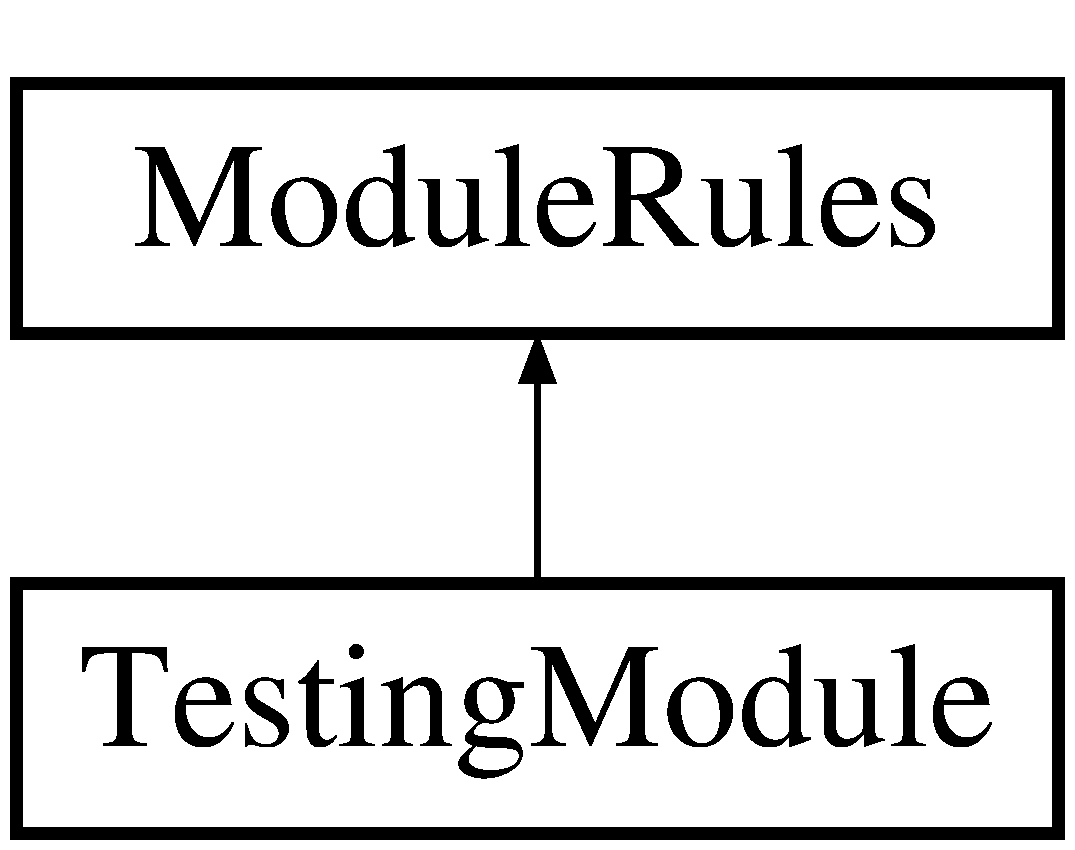
\includegraphics[height=2.000000cm]{class_testing_module}
\end{center}
\end{figure}
\subsection*{Public Member Functions}
\begin{DoxyCompactItemize}
\item 
\mbox{\Hypertarget{class_testing_module_aa52e5bcee3093b473e13827ab5fdfe5d}\label{class_testing_module_aa52e5bcee3093b473e13827ab5fdfe5d}} 
{\bfseries Testing\+Module} (Read\+Only\+Target\+Rules Target)
\end{DoxyCompactItemize}


The documentation for this class was generated from the following file\+:\begin{DoxyCompactItemize}
\item 
Source/\+Testing\+Module/Testing\+Module.\+Build.\+cs\end{DoxyCompactItemize}

%--- End generated contents ---

% Index
\backmatter
\newpage
\phantomsection
\clearemptydoublepage
\addcontentsline{toc}{chapter}{Index}
\printindex

\end{document}
